\section{Outils et Procédures de Décompression}

\begin{frame}{Objectifs et Introduction}
    \begin{itemize}
        \item Apprendre à utiliser et paramétrer son moyen de décompression.
        \item Savoir planifier une plongée avec son ordinateur.
        \item Comprendre les protocoles de secours (Tables MN90).
        \item Gérer la cohabitation de différents ordinateurs au sein de la palanquée.
    \end{itemize}
\end{frame}

\begin{frame}{Objectifs : Gestion de la Décompression N3}
    \small
    Dans le cadre de l'autonomie N3, l'objectif est d'assurer une décompression optimale et sécurisée pour l'ensemble de la palanquée.

    \vspace{0.3cm}

    \begin{itemize}
        \item \textbf{Compréhension et Maîtrise de l'Ordinateur :}
        \begin{itemize}
            \item Connaître succinctement les modèles de désaturation (avantages/limites).
            \item Maîtriser les réglages (Durcissement, \% $O_2$, etc.).
            \item Savoir \textbf{planifier} une plongée avant l'immersion.
        \end{itemize}

        \vspace{0.2cm}

        \item \textbf{Gestion de la Palanquée (Cohabitation) :}
        \begin{itemize}
            \item Prendre en compte la diversité des ordinateurs.
            \item Harmoniser les procédures de désaturation entre équipiers.
        \end{itemize}

        \vspace{0.2cm}

        \item \textbf{Procédures de Secours :}
        \begin{itemize}
            \item Utiliser les \textbf{Tables Fédérales (MN90)} en cas de défaillance électronique.
        \end{itemize}
    \end{itemize}
\end{frame}

\begin{frame}{Rappel : Courbe de Sécurité}
    \textbf{Définition :}
    La courbe de sécurité indique, pour chaque profondeur, le temps maximum de plongée réalisable sans avoir à effectuer de paliers de décompression obligatoires.

    \vspace{0.5cm}
    \centering
    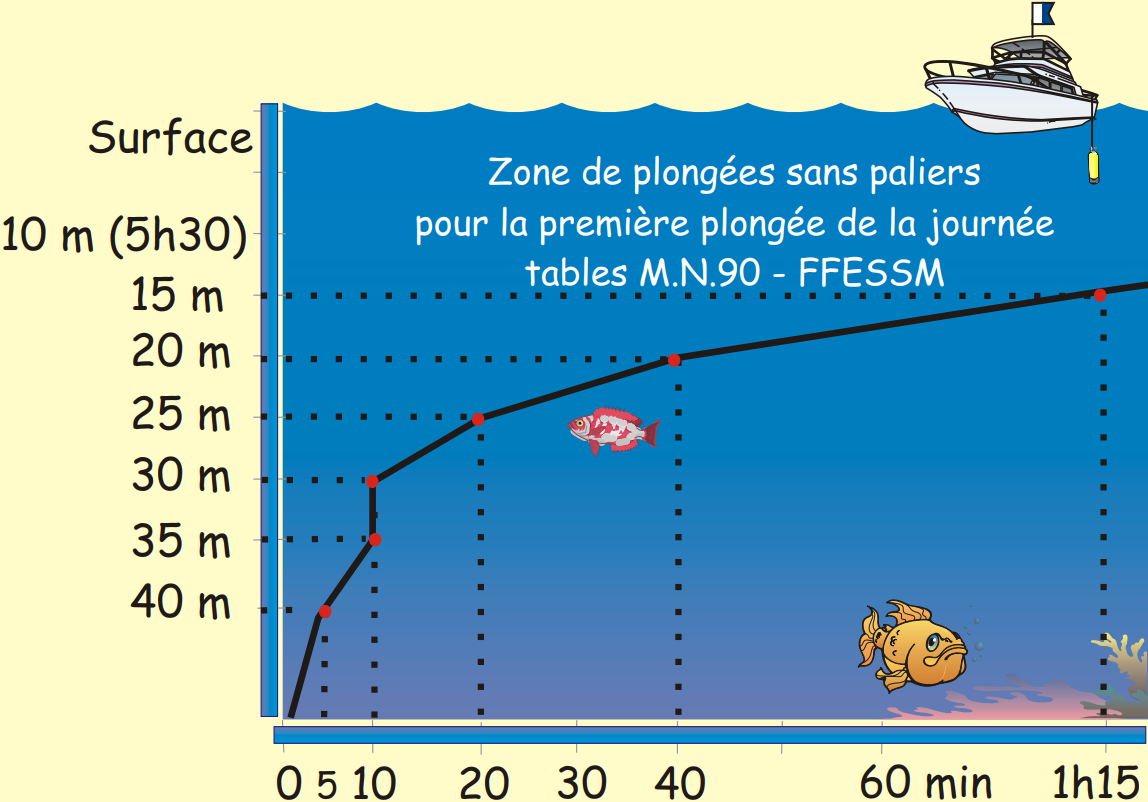
\includegraphics[height=0.65\textheight, keepaspectratio]{images/courbe_securite.png}
\end{frame}

\begin{frame}{Tables MN90 : Principes et Plongée Simple}
    \textbf{Présentation de l'outil :}
    \begin{itemize}
        \item Tables "Loisir" basées sur un profil carré (2 plongées/24h).
        \item \textbf{Vitesse de remontée :} 15 à 17 m/min.
        \item \textbf{Vitesse inter-paliers :} 6 m/min.
    \end{itemize}

    \vspace{0.3cm}

    \begin{block}{Règles de la Plongée Simple (Intervalle $>12h$)}
        \begin{itemize}
            \item \textbf{Profondeur :} Retenir la profondeur \textbf{maximale} atteinte.
            \item \textbf{Durée :} Du début de l'immersion jusqu'au \textbf{début de la remontée} (à 15-17 m/min).
            \item \textbf{Lecture :} Si la valeur exacte n'existe pas, prendre toujours la \textbf{valeur immédiatement supérieure}.
        \end{itemize}
    \end{block}
\end{frame}

\begin{frame}{Exemple d'Application : Lecture de Table et Remontée Lente}
    \begin{columns}
        \begin{column}{0.65\textwidth}
            \centering
            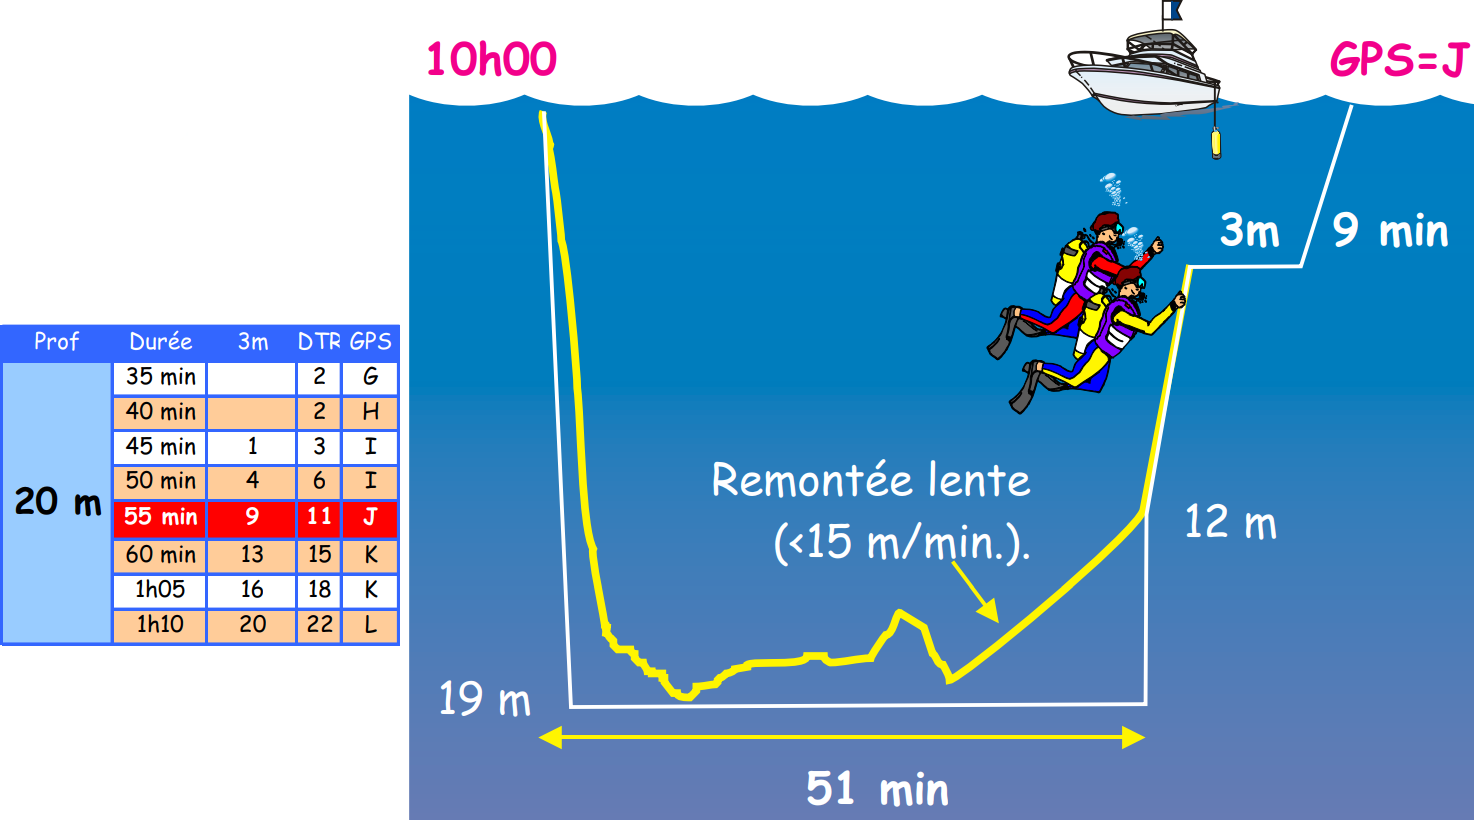
\includegraphics[width=\columnwidth]{images/table_mn90_exemple_1}
        \end{column}

        % COLONNE DROITE : EXPLICATION PAS À PAS
        \begin{column}{0.35\textwidth}
            \small
            \textbf{Analyse du profil :}
            \begin{enumerate}
                \item \textbf{Profondeur :} \\
                $19\text{m} \rightarrow$ On lit la table \textbf{20m}.
                
                \item \textbf{Durée :} \\
                Remontée lente ($<15$m/min) $\rightarrow$ La durée inclut la remontée. \\
                Temps retenu : \textbf{51 min}.
                
                \item \textbf{Lecture :} \\
                $51$ min n'est pas dans la table. \\
                $\rightarrow$ On prend le supérieur : \textbf{\textcolor{red}{55 min}}.
            \end{enumerate}

            
            \textbf{Résultat (Ligne 55') :}
            \begin{itemize}
                \item \textbf{Paliers :} 9 min à 3m.
                \item \textbf{GPS :} Lettre J.
            \end{itemize}
        \end{column}
    \end{columns}
\end{frame}

\begin{frame}{Les Plongées Successives : Mécanisme Global}
    \vspace{-0.4cm} 
    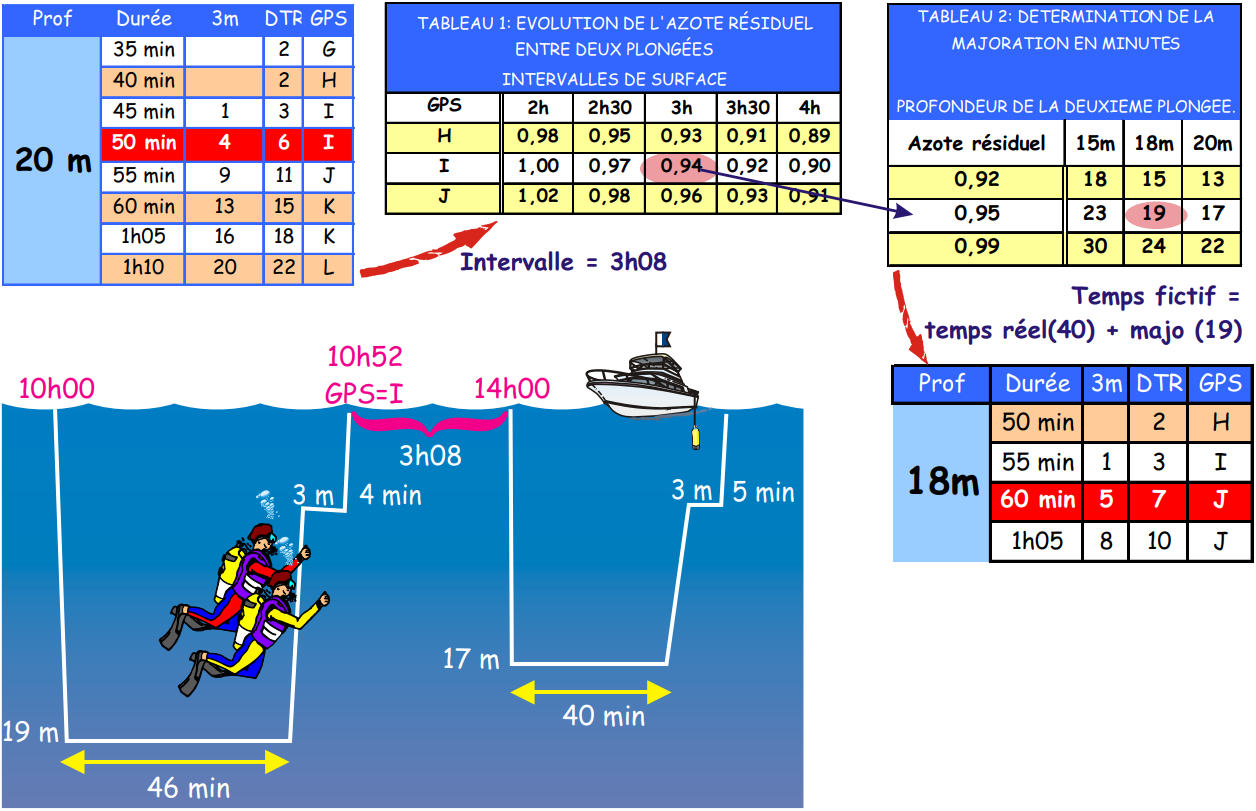
\includegraphics[height=0.85\textheight, keepaspectratio]{images/table_mn90_exemple_2_plongee.png}

    \vspace{-2cm} 

    \hfill
    \fcolorbox{red}{white}{
        \begin{minipage}{0.45\textwidth} % Largeur du bloc de texte
            \centering
            \textbf{\textcolor{red}{Règle pour la 2\textsuperscript{ème} plongée :}} \\[0.1cm]
            \large $\text{Temps Fictif} = \text{T. Réel} + \text{Majoration}$
        \end{minipage}
    }
\end{frame}
\begin{frame}{Tables MN90 : Procédures Anormales}
    
    \begin{alertblock}{1. Remontée Rapide ($>$ 15 à 17 m/min)}
        \begin{enumerate}
            \item \textbf{$<$ 3 min} : Redescendre à \textbf{mi-profondeur}.
            \item Y rester \textbf{5 min} (stabilisation).
            \item \textbf{Recalcul des paliers :} 
            \begin{itemize}
                \item Profondeur Max + Durée Totale (incluant les 5 min).
            \end{itemize}
            \item \textbf{Impératif :} Minimum 2 min à 3m (même si table = 0).
        \end{enumerate}
    \end{alertblock}

    \vspace{0.5cm}

    \begin{block}{2. Interruption de Palier}
        \begin{itemize}
            \item \textbf{$<$ 3 min} pour se réimmerger.
            \item \textbf{Reprendre le palier à zéro} (recommencer en totalité).
        \end{itemize}
    \end{block}
\end{frame}

\begin{frame}{Transition : De la Table à l'Ordinateur}
    \footnotesize
    \begin{columns}[c]
        \begin{column}{0.5\textwidth}
            \centering
            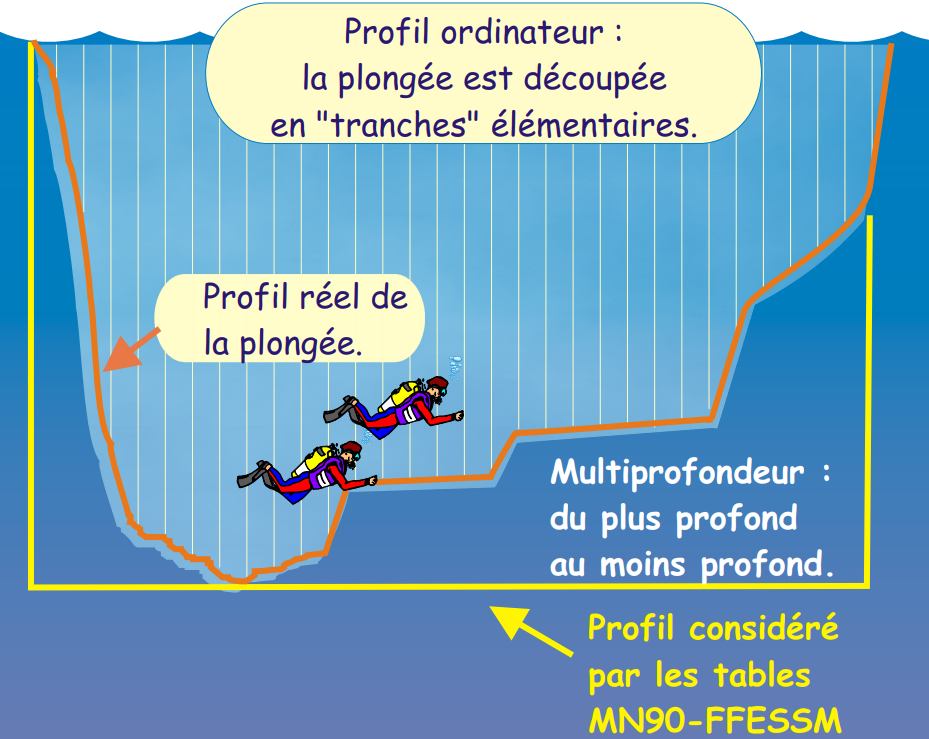
\includegraphics[width=\columnwidth]{images/table_vs_ordinateur}
        \end{column}

        \begin{column}{0.5\textwidth}
            \textbf{La Logique des Tables :}
            \begin{itemize}
                \setlength\itemsep{0em}
                \item Elles considèrent un \textbf{profil carré}.
                \item Hypothèse : Tout le temps de plongée est passé à la profondeur \textbf{maximale}.
                \item \textit{Conséquence :} Pénalisant pour les plongées multi-niveaux.
            \end{itemize}

            \textbf{La Logique de l'Ordinateur :}
            \begin{itemize}
                \setlength\itemsep{0em}
                \item Il suit le \textbf{profil réel} (ligne orange).
                \item Calcul dynamique : La plongée est découpée en "tranches" élémentaires pour ajuster la saturation en temps réel.
            \end{itemize}
            \vspace{-0.1cm}
            \begin{exampleblock}{Le Bénéfice pour le Plongeur N3}
                L'ordinateur optimise le temps de plongée sans palier (courbe de sécurité) en prenant en compte la remontée progressive.
            \end{exampleblock}
        \end{column}
    \end{columns}
\end{frame}

\begin{frame}{L'Ordinateur de Plongée — Réglages}
    L'ordinateur calcule la saturation en temps réel. Attention aux réglages avant la mise à l'eau :
    \begin{itemize}
        \item \textbf{Le Mélange} : Air ou Nitrox. \textit{\textcolor{ffessmred}{Danger} : Un ordi réglé sur Nitrox 
            pour une plongée à l'air indiquera moins de paliers que nécessaire}.
        \item \textbf{L'Altitude} : Au-dessus de 300m, les procédures changent (automatique ou manuel).
        \item \textbf{Les Alarmes} : Ne pas ignorer les alarmes sonores (vitesse de remontée, paliers).
        \item \textbf{La Dureté} : Possibilité de durcir les paliers pour plus de sécurité 
            (facteurs de risque).
    \end{itemize}
\end{frame}

\begin{frame}{L'Ordinateur de Plongée — Planification et Gestion de Palanquée}
    \textbf{Le Rôle de l'Ordinateur :}
    \begin{itemize}
        \item \textbf{Mode "PLAN" :} Il utilise l'historique de vos plongées précédentes pour simuler la suivante.
        \item \textbf{Objectif :} Définir un profil pour rester dans la courbe de sécurité (sans palier) ou planifier la durée des paliers acceptés.
    \end{itemize}

    \vspace{0.3cm}

    \begin{block}{La Cohabitation (Accord au sein de la palanquée)}
        Avant de s'immerger, il est crucial d'harmoniser les instruments de la palanquée :
        \begin{itemize}
            \item \textbf{Comparer les paramètres :} Qui a le profil le plus restrictif ?
            \item \textbf{Comprendre l'autre ordi :} Sait-on lire les infos du binôme ?
            \item \textbf{Protocoles spécifiques :} L'un des ordinateurs impose-t-il des paliers profonds ou facultatifs ?
        \end{itemize}
        \textbf{$\rightarrow$ On s'accorde en surface sur la conduite à tenir.}
    \end{block}
\end{frame}

\begin{frame}{L'Ordinateur de Plongée — Limites et Précautions d'Usage}
    \begin{columns}[t]
        \begin{column}{0.48\textwidth}
            \begin{alertblock}{Les Limites de la Machine}
                L'ordinateur calcule une saturation théorique mais \textbf{ne connait pas votre état} :
                \begin{itemize}
                    \item Froid, fatigue, stress ?
                    \item Consommation d'air ?
                    \item Forme physique ?
                \end{itemize}
                \textit{Le plongeur N3 doit garder son discernement et durcir les paliers si nécessaire.}
            \end{alertblock}
        \end{column}

        \begin{column}{0.48\textwidth}
            \textbf{Consignes Avant Immersion :}
            \begin{itemize}
                \item \textbf{Instrument Personnel :} Ne jamais prêter ou échanger un ordinateur en cours de série (il contient VOTRE saturation).
                \item \textbf{Vérification des Réglages :}
                \begin{itemize}
                    \item Est-il en mode \textbf{Nitrox} ou Air ? (Risque d'erreur de calcul).
                    \item Est-il en mode \textbf{Gauge/Profondimètre} ? (Pas de calcul de désaturation !).
                \end{itemize}
            \end{itemize}
        \end{column}
    \end{columns}
\end{frame}

\begin{frame}{Précautions — Ne pas "jouer" avec la Courbe de Sécurité}
    \begin{alertblock}{Comportement à Risque : "Surfer sur la limite"}
        Il est dangereux de flirter avec la limite de non-décompression (NDL) affichée par l'ordinateur.
        
        \vspace{0.5em}
        \textbf{Le scénario à éviter absolument :}
        \begin{enumerate}
            \item Attendre que le temps sans palier affiche \textbf{0 min}.
            \item Remonter de quelques mètres juste pour récupérer \textbf{1 ou 2 min} de "rab".
            \item Rester à cette nouvelle profondeur jusqu'à retomber à \textbf{0 min}.
            \item Répéter l'opération...
        \end{enumerate}
    \end{alertblock}

    \textbf{Pourquoi est-ce dangereux ?}
    \begin{itemize}
        \item Vous saturez votre organisme au \textbf{maximum théorique} acceptable par le modèle mathématique.
        \item Vous ne laissez aucune marge pour les imprévus (effort, froid, erreur de vitesse).
        \item En cas de remontée rapide accidentelle ou d'effort, l'accident est quasi inévitable.
    \end{itemize}
\end{frame}

\begin{frame}{Précautions — La Règle de Sécurité N3}
    Face à ces limites théoriques, le Plongeur N3 doit adopter une attitude responsable.

    \vspace{0.5cm}

    \begin{exampleblock}{La Bonne Pratique : La Marge de Sécurité}
        Il ne faut jamais attendre que l'ordinateur affiche zéro.
        
        \vspace{0.3cm}
        \centering
        \textbf{La Règle :} \\
        Décider de quitter le fond (ou remonter franchement) lorsqu'il reste encore : \\
        \huge \textcolor{blue}{3 à 5 minutes} \\
        \normalsize avant l'affichage des paliers obligatoires.
    \end{exampleblock}

    \vspace{0.5cm}
    \small
    \textit{Cette marge permet de compenser les facteurs non pris en compte par l'ordinateur (froid, fatigue, âge, forme physique).}
\end{frame}

\begin{frame}{Procédure Ordinateur : Vitesse de Remontée Trop Rapide}
    \small
    \textbf{Définition :} Vitesse $> 15$ m/min, entre 30m et surface, sur $\ge 10$m.

    \begin{block}{Si la ré-immersion est possible ($<$ 3 min)}
        \begin{enumerate}
            \item Redescendre au moins à \textbf{mi-profondeur}.
            \item Y effectuer un palier de \textbf{5 minutes}.
            \item Remonter et faire \textbf{au moins} (en plus des paliers ordi) :
            \begin{itemize}
                \item \textbf{1 minute à 6 mètres}.
                \item \textbf{5 minutes à 3 mètres}.
            \end{itemize}
        \end{enumerate}
    \end{block}

    \begin{alertblock}{Si la ré-immersion est IMPOSSIBLE}
        \begin{itemize}
            \item Mise sous \textbf{Oxygène}.
            \item \textbf{Évacuation} vers un centre hyperbare.
        \end{itemize}
    \end{alertblock}
\end{frame}

\begin{frame}{Procédure Ordinateur : Palier Obligatoire Non-Réalisé}
    \small
    \begin{block}{Si la ré-immersion est possible ($<$ 3 min)}
        \begin{itemize}
            \item Se réimmerger immédiatement.
            \item Suivre les indications du moyen de décompression.
            \item \textbf{Rajouter 3 minutes à 3 mètres} (quel que soit le temps manqué).
        \end{itemize}
    \end{block}
    \vspace{-0.1cm}
    \begin{alertblock}{Si la ré-immersion est IMPOSSIBLE}
        \textbf{Déclenchement des SECOURS (O2 + Évacuation)}
        \begin{itemize}
            \item Si \textbf{signe} d'accident éventuel.
            \item OU si durée des paliers non-réalisés \textbf{$>$ 3 minutes}.
        \end{itemize}
        
        \textbf{Surveillance (Mise en observation)}
        \begin{itemize}
            \item Si durée des paliers non-réalisés \textbf{$\le$ 3 minutes} (ET aucun signe).
            \item \textbf{Protocole :} Observation pendant \textbf{3 heures} + Interdiction de plongée \textbf{24h}.
        \end{itemize}
    \end{alertblock}
\end{frame}

\begin{frame}{Exercice 1 : Lecture d'Ordinateur (Mares Couleur)}
    \begin{columns}
        % Colonne Image
        \column{0.45\textwidth}
            \centering
            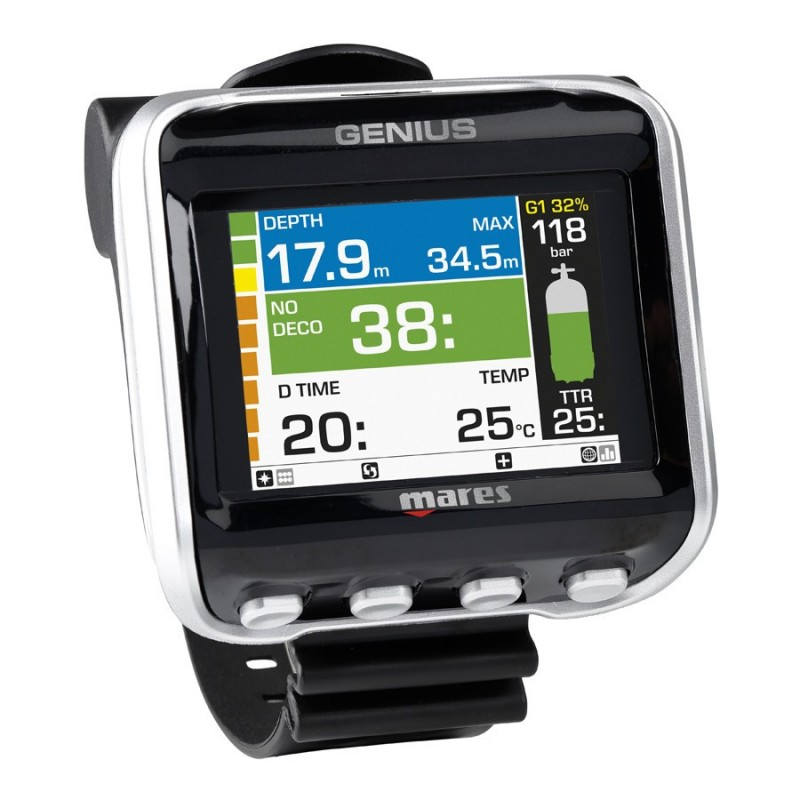
\includegraphics[width=\columnwidth, keepaspectratio]{images/schema_ordi_2}

        \column{0.5\textwidth}
            \only<1>{
                \textbf{Analysez cet écran :}
                \begin{enumerate}
                    \item Quelle est la profondeur actuelle ?
                    \item Quelle est la profondeur max ?
                    \item Statut : Courbe de sécurité ou Décompression ?
                    \item Que signifie le chiffre \textbf{38} (NO DECO) ?
                    \item Quel gaz respire le plongeur ?
                    \item Que signifie \textbf{TTR 25} ?
                \end{enumerate}
            }

            \only<2>{
                \begin{exampleblock}{Analyse : Paramètres et Gestion d'Air}
                    \begin{itemize}
                        \item \textbf{Actuelle :} 17,9 m / \textbf{Max :} 34,5 m.
                        \item \textbf{Statut :} NO DECO (Pas de palier).
                        \item \textbf{NDL (38 min) :} Temps restant sans palier obligatoire.
                        \item \textbf{Gaz :} \textbf{Nitrox 32\%} (G1 32\% en haut à droite).
                        \item \textbf{Pression :} 118 bar.
                        \item \textbf{TTR (25 min) :} \textit{Time To Reserve}. 
                        Temps restant avant d'atteindre la réserve (basé sur la conso actuelle), différent de la DTR !
                    \end{itemize}
                \end{exampleblock}
            }
    \end{columns}
\end{frame}

\begin{frame}{Exercice 2 : Lecture d'Ordinateur (Mares LCD)}
    \begin{columns}
        \column{0.45\textwidth}
            \centering
            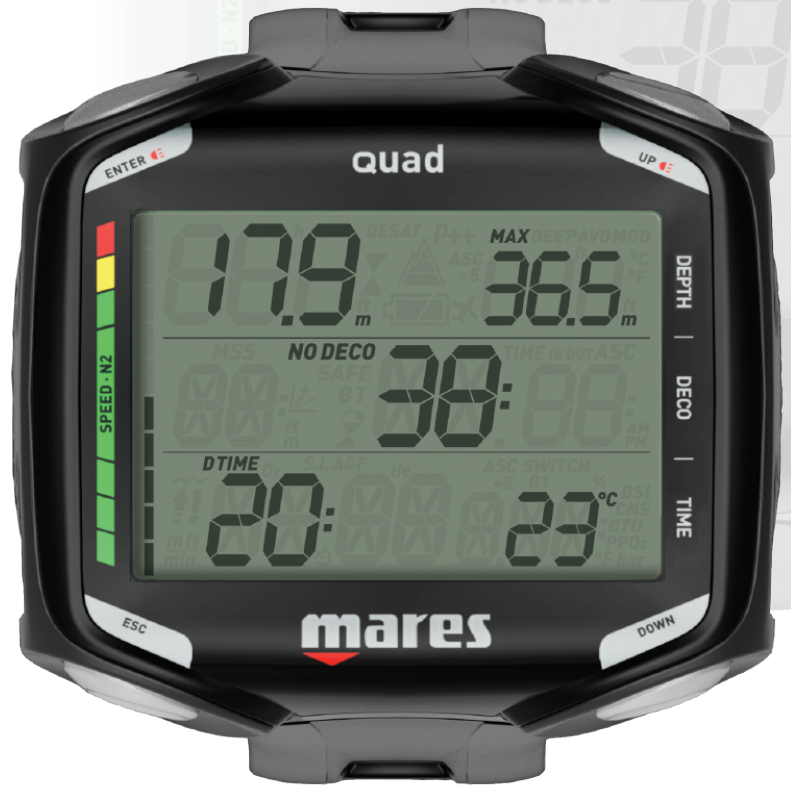
\includegraphics[width=\columnwidth, keepaspectratio]{images/schema_ordi_3}

        \column{0.5\textwidth}
            \only<1>{
                \textbf{Analysez cet écran :}
                \begin{enumerate}
                    \item Quelle est la profondeur actuelle ?
                    \item Quelle est la profondeur max ?
                    \item Statut : Courbe de sécurité ou Décompression ?
                    \item Combien de temps peut-on encore rester à cette profondeur sans palier ?
                    \item Quelle est la durée de plongée écoulée ?
                    \item Quelle est la température de l'eau ?
                \end{enumerate}
            }

            \only<2>{
                \begin{exampleblock}{Analyse : Dans la Courbe}
                    \begin{itemize}
                        \item \textbf{Actuelle :} 17,9 m.
                        \item \textbf{Max :} 36,5 m.
                        \item \textbf{Statut :} NO DECO.
                        \item \textbf{NDL (38 min) :} "No Deco Limit". Temps restant sans palier obligatoire.
                        \item \textbf{DTIME (20 min) :} Temps de plongée écoulé.
                        \item \textbf{Température :} 23$^\circ$C.
                    \end{itemize}
                \end{exampleblock}
            }
    \end{columns}
\end{frame}

\begin{frame}{Exercice 3 : Lecture d'Ordinateur (Situation Déco)}
    \begin{columns}
        \column{0.45\textwidth}
            \centering
            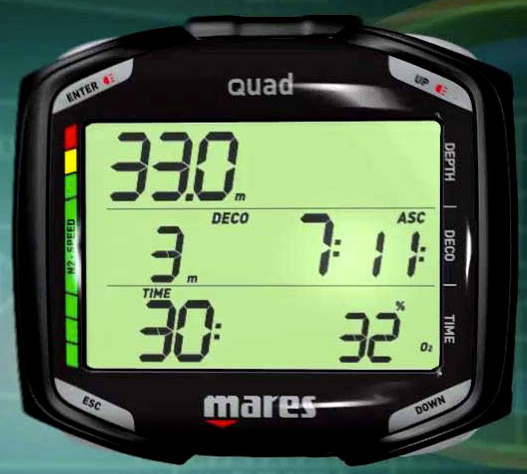
\includegraphics[width=\columnwidth, keepaspectratio]{images/schema_ordi_4}

        \column{0.5\textwidth}
            \only<1>{
                \textbf{\textcolor{red}{Attention, situation différente !}}
                \begin{enumerate}
                    \item Quelle est la profondeur actuelle ?
                    \item Sommes-nous en décompression ?
                    \item Quelle est la profondeur du palier obligatoire ?
                    \item Quelle est la durée de ce palier ?
                    \item Quel est le temps total de remontée (ASC) ?
                    \item Quel est le mélange respiré ?
                \end{enumerate}
            }

            \only<2>{
                \begin{alertblock}{Analyse : Paliers Obligatoires}
                    \begin{itemize}
                        \item \textbf{Actuelle :} 33,0 m.
                        \item \textbf{Statut :} DECO.
                        \item \textbf{Prof. Palier :} 3 m.
                        \item \textbf{Durée :} 7 min.
                        \item \textbf{ASC (11 min) :} "Ascent Time" (DTR). Temps total pour sortir (Remontée + Paliers).
                        \item \textbf{Gaz :} \textbf{Nitrox 32\%}.
                    \end{itemize}
                \end{alertblock}
            }
    \end{columns}
\end{frame}

\begin{frame}{Exercice 4 : Lecture d'Ordinateur (Suunto)}
    \begin{columns}
        \column{0.45\textwidth}
            \centering
            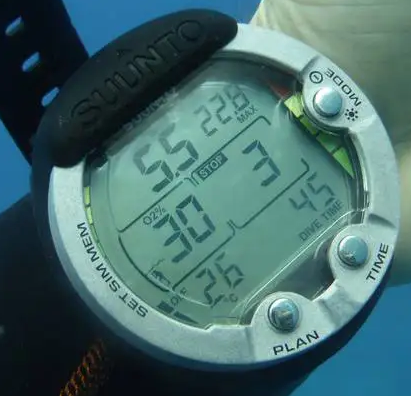
\includegraphics[width=\columnwidth, keepaspectratio]{images/schema_ordi_1}

        \column{0.5\textwidth}
            \only<1>{
                \textbf{Analysez cet écran :}
                \begin{enumerate}
                    \item Quelle est la profondeur actuelle ?
                    \item Quelle est la profondeur max ?
                    \item Y a-t-il un palier à faire ? À quelle profondeur ?
                    \item Quel est le mélange respiré ?
                    \item Quelle est la durée de la plongée ?
                \end{enumerate}
            }

            \only<2>{
                \begin{block}{Analyse : Fin de Plongée / Palier}
                    \begin{itemize}
                        \item \textbf{Actuelle :} 5,5 m.
                        \item \textbf{Max :} 22,8 m.
                        \item \textbf{Palier :} OUI (Icône \textbf{STOP}). Plafond à \textbf{3 m}.
                        \item \textbf{Gaz :} \textbf{Nitrox 30\%}.
                        \item \textbf{Durée :} 45 min.
                    \end{itemize}
                    \vspace{0.2cm}
                    \scriptsize \textit{Note : Sur ce modèle, l'affichage "STOP" avec une profondeur indique une obligation de s'arrêter (palier obligatoire ou de sécurité activé).}
                \end{block}
            }
    \end{columns}
\end{frame}

\begin{frame}{Exercice 5 : Lecture d'Ordinateur (Shearwater)}
    \begin{columns}
        \column{0.45\textwidth}
            \centering
            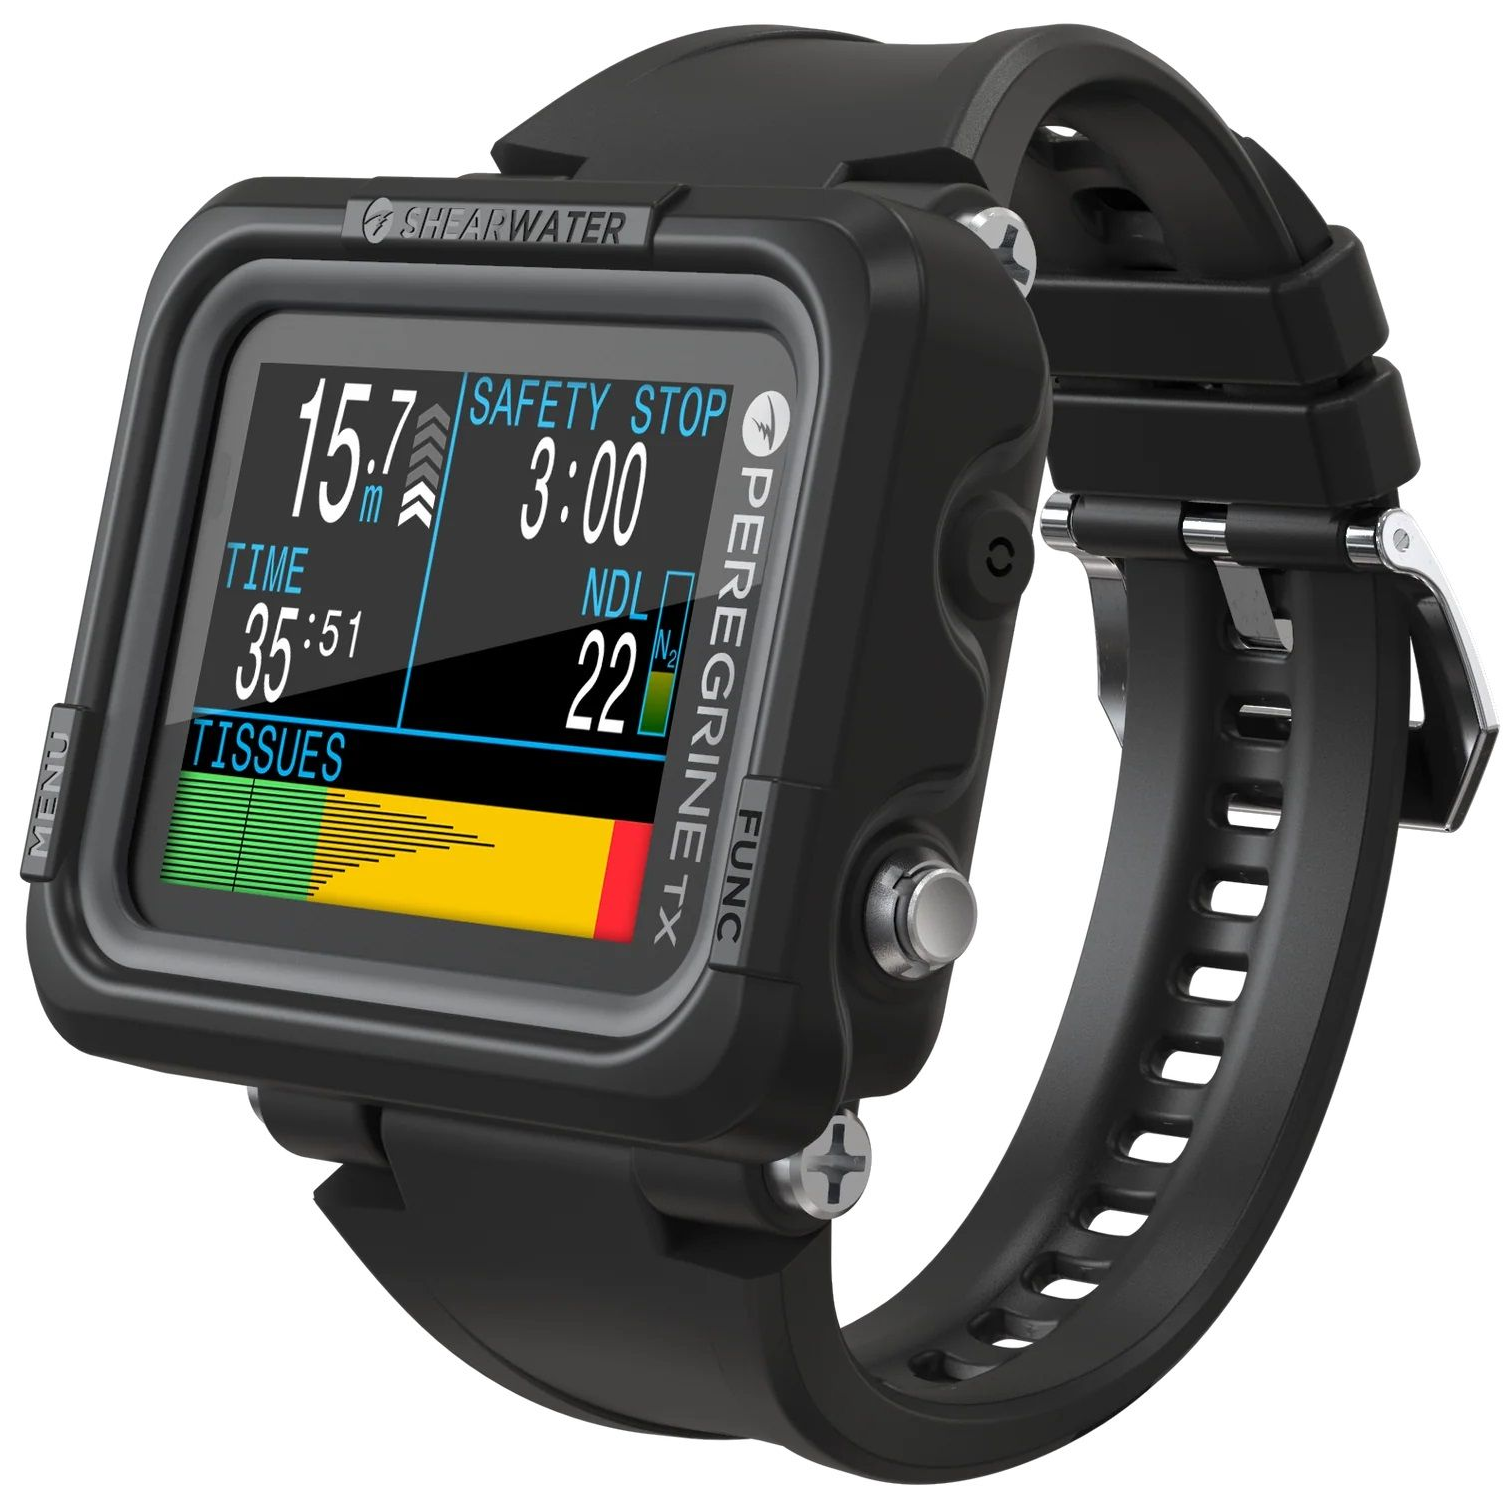
\includegraphics[width=\columnwidth, keepaspectratio]{images/schema_ordi_5}

        \column{0.55\textwidth}
            \only<1>{
                \textbf{Analysez cet écran (OLED Couleur) :}
                \begin{enumerate}
                    \item Quelle est la profondeur actuelle ?
                    \item Combien de temps reste-t-il avant d'avoir des paliers (NDL) ?
                    \item Que signifie "SAFETY STOP 3:00" ?
                    \item Que représente le graphique en bas ("TISSUES") ?
                    \item \textbf{Que représente la barre verticale avec les flèches ?}
                \end{enumerate}
            }

            \only<2>{
                \begin{exampleblock}{Analyse : Interface Graphique}
                    \begin{itemize}
                        \item \textbf{Actuelle :} 15,7 m.
                        \item \textbf{NDL (22 min) :} Temps restant sans palier ("No Decompression Limit").
                        \item \textbf{Safety Stop :} Palier de sécurité (facultatif) prévu de 3 min.
                        \item \textbf{Tissues :} Visualisation de la saturation des 16 compartiments théoriques.
                        \item \textbf{Vitesse de Remontée :} La barre latérale est un variomètre. 
                        La flèche monte et la barre change de couleur (Jaune $\rightarrow$ Rouge) 
                        si la vitesse de remontée est trop rapide.
                    \end{itemize}
                \end{exampleblock}
            }
    \end{columns}
\end{frame}

\begin{frame}{Exercice 6 : Lecture d'Ordinateur (Aqualung)}
    \begin{columns}
        \column{0.45\textwidth}
            \centering
            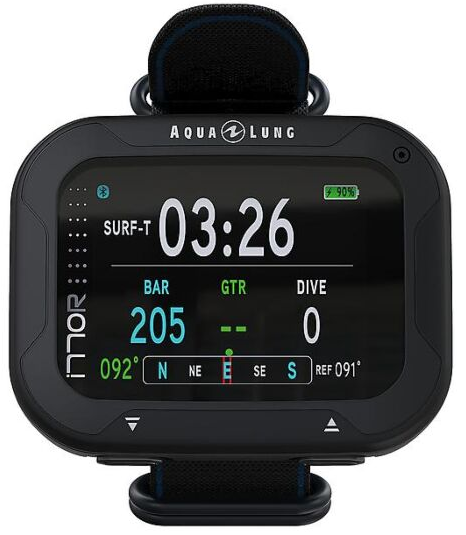
\includegraphics[width=0.9\columnwidth, keepaspectratio]{images/schema_ordi_6}

        \column{0.55\textwidth}
            \only<1>{
                \textbf{Analysez cet écran (TFT Couleur) :}
                \begin{enumerate}
                    \item À quelle profondeur se trouve le plongeur ?
                    \item Que signifie \textbf{SURF-T} ?
                    \item Quelle est la pression dans la bouteille ?
                    \item Quelle est l'orientation indiquée par le compas ?
                    \item Pourquoi "DIVE" indique 0 ?
                \end{enumerate}
            }

            \only<2>{
                \begin{alertblock}{Analyse : Mode SURFACE}
                    \textbf{Attention, nous ne sommes pas sous l'eau !}
                    \begin{itemize}
                        \item \textbf{Profondeur :} 0 m (Nous sommes en surface).
                        \item \textbf{SURF-T (03:26) :} \textit{Surface Time}. Intervalle de surface depuis la dernière plongée (3h 26min).
                        \item \textbf{Pression :} 205 Bar (Prêt à partir !).
                        \item \textbf{Compas :} Cap 92° (Est).
                        \item \textbf{DIVE 0 :} Le temps de plongée est à zéro car l'immersion n'a pas commencé.
                    \end{itemize}
                \end{alertblock}
            }
    \end{columns}
\end{frame}